\chapter{State of Artificial Intelligence}

%-------------------------------------------------------------
\section{Introduction}

This chapter presents the key technologies underlying modern intelligent
question-answering applications. It covers Large Language Models, their
capabilities and limitations, the Retrieval-Augmented Generation architecture
that addresses those limitations, and the evaluation framework used to measure
performance and response quality.

%-------------------------------------------------------------
\section{Large Language Model}
%-------------------------------------------------------------

In this section, we discuss Large Language Models (LLMs), covering their
definition, history, types, training phases, common applications,
and their limitations.

%-------------------------------------------------------------
\subsection{Presentation}
%-------------------------------------------------------------

Large Language Models (LLMs) are AI systems based on deep neural networks
trained on large datasets to understand and generate natural language.
They use the transformer architecture, which is efficient for processing
text sequences and capturing context~\cite{ialayers}.

\textbf{Figure~2.1}~\cite{ialayers} shows the layers of Artificial Intelligence.

\begin{figure}[H]
\centering
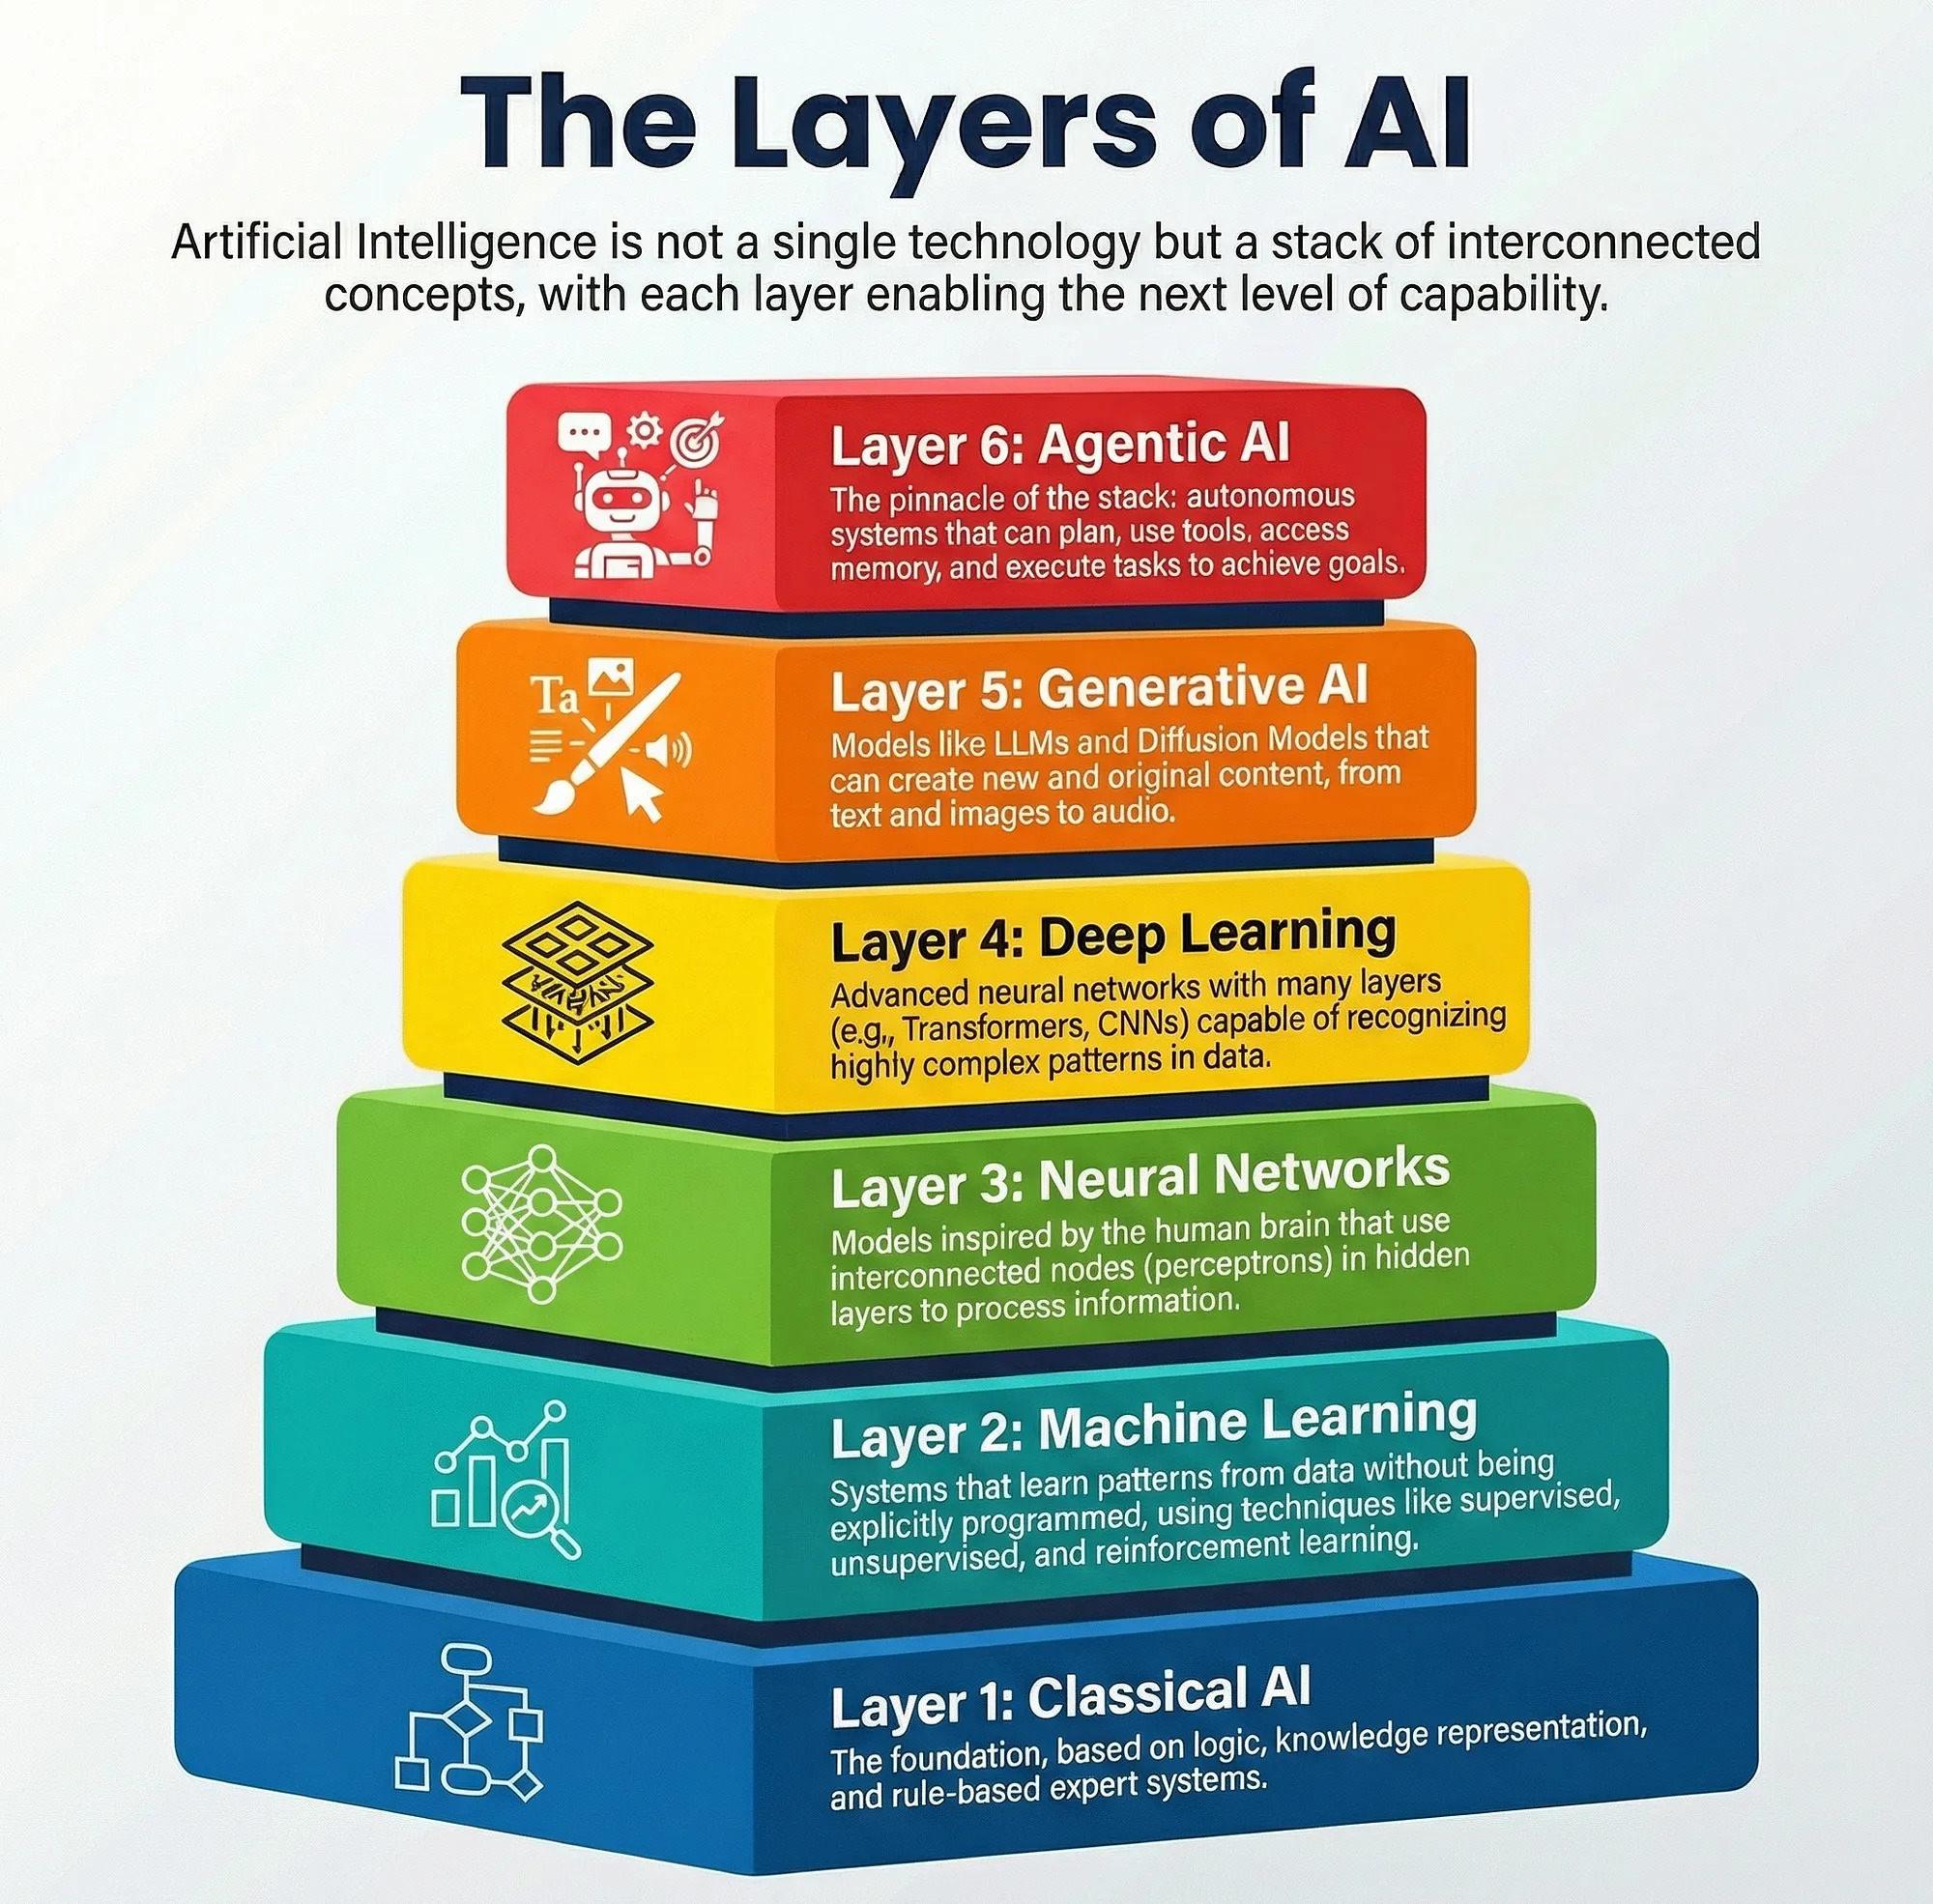
\includegraphics[width=0.5\textwidth]{ia_layers.jpg}
\caption{The Field of Artificial Intelligence: Layer by Layer~\cite{ialayers}}
\end{figure}

The history of LLMs began in the 1950s with early Natural Language
Processing (NLP) research and systems such as machine translation and ELIZA,
which demonstrated basic human-computer interaction. Progress accelerated
with the introduction of neural networks and LSTM models in the 1990s,
followed by major NLP advances such as Word2Vec and CoreNLP in the 2010s.
A major breakthrough occurred in 2017 with the Transformer architecture,
which significantly improved language modelling performance, leading to
models such as BERT in 2018. Finally, the release of ChatGPT in 2022
marked a major milestone, making LLMs widely accessible and accelerating
their adoption in real-world applications.

LLMs can be categorised into three types: pre-trained models, fine-tuned
models, and multimodal models. Each type offers advantages depending on
the desired outcome, as summarised in Table \textbf{2.1}.

\begin{table}[H]
\centering
\caption{Types of Large Language Models}
\label{tab:llm-types}
\renewcommand{\arraystretch}{1.5}

\begin{tabular}{|p{3.5cm}|p{5cm}|p{3.5cm}|p{3.5cm}|}
\hline
\textbf{Type} & \textbf{Description} & \textbf{Examples} & \textbf{Best For} \\
\hline
Pre-trained Models &
Trained on massive general datasets; understand and generate text
for a wide range of tasks. &
GPT-4, LLaMA 2, BLOOM &
General-purpose NLP tasks \\
\hline

Fine-tuned Models &
Built on a pre-trained base and further trained on domain-specific
data for targeted tasks. &
Vicuna, CodeGen, fine-tuned BERT &
Domain-specific tasks (legal, medical, code) \\
\hline

Multimodal Models &
Process text, images, audio, and video simultaneously, making them
significantly more capable. &
GPT-4V, Gemini, Claude 3 &
Visual QA, transcription, rich media analysis \\
\hline
\end{tabular}
\end{table}


Large Language Models are widely used in various domains due to their
versatility and ability to process natural language efficiently.

\begin{itemize}
  \item \textbf{Chatbots and Virtual Assistants:} LLMs are used to build
        intelligent conversational agents capable of interacting with users
        in natural language.
  \item \textbf{Text Generation:} Automatic generation of articles, reports,
        and summaries.
  \item \textbf{Machine Translation:} Translating text between multiple
        languages with high accuracy.
  \item \textbf{Code Generation:} Assisting developers by generating and
        explaining code.
  \item \textbf{Information Retrieval:} Enhancing search engines by
        understanding user queries semantically.
\end{itemize}

While LLMs offer broad capabilities, selecting the right model for a
specific application requires a structured comparison. The following
subsection examines the most relevant models and the criteria used
to guide this choice.

%-------------------------------------------------------------
\subsection{Choice of LLM}
%-------------------------------------------------------------

\subsubsection{a- The Most Popular Large Language Models}

The ecosystem of Large Language Models has developed quickly in recent years,
with several organisations offering powerful models accessible through APIs.
These models are widely adopted in real-world applications due to their
scalability, high performance, and ease of integration into intelligent
systems such as chatbots and Retrieval-Augmented Generation (RAG) applications.
Table \textbf{2.2} presents some of the most widely used API-based
Large Language Models and their main strengths.

\begin{table}[H]
\centering
\caption{Popular API-based Large Language Models}
\label{tab:llm_popular}
\begin{tabular}{|p{4cm}|p{3cm}|p{3cm}|p{5cm}|}
\hline
\textbf{Model} & \textbf{Provider} & \textbf{Type} & \textbf{Key Strengths} \\
\hline

GPT-4 / GPT-4.1 &
OpenAI &
Multimodal &
High accuracy, strong reasoning, excellent for RAG and complex queries \\
\hline

Claude Sonnet 4.0 &
Anthropic &
Multimodal &
Long context window, safe outputs, strong reasoning and document analysis \\
\hline

Gemini 1.5 Pro &
Google &
Multimodal &
Very large context window (up to 1M tokens), ideal for long documents \\
\hline

Mistral Large &
Mistral AI &
Text-based &
Fast, cost-efficient, strong performance in structured tasks \\
\hline

LLaMA 3 (API via providers) &
Meta / Groq / Together AI &
Text-based &
Open ecosystem, flexible deployment, good balance between performance
and cost \\
\hline

\end{tabular}
\end{table}

The large variety of available LLMs makes model selection a challenging task.
Therefore, defining clear evaluation criteria is essential to identify the
most suitable model for the target application.

%-------------------------------------------------------------

\subsubsection{b- Criteria for Choosing the Right Large Language Model}

Choosing the right Large Language Model means selecting the model that best
satisfies the technical, functional, and operational requirements of the system.
Table~\ref{tab:llm_criteria} presents the main criteria used in this
comparative study.

\begin{table}[H]
\centering
\caption{LLM Selection Criteria}
\label{tab:llm_criteria}
\begin{tabular}{|p{5cm}|p{9cm}|}
\hline
\textbf{Criteria} & \textbf{Description} \\
\hline

Accuracy \& Reliability &
Hallucination rate, citation precision, contextual fidelity,
numerical accuracy \\
\hline

Context Window &
Maximum tokens supported and long-context understanding \\
\hline

Multilingual Capability &
Support for French, English, Arabic, and multilingual reasoning \\
\hline

Domain Expertise &
Knowledge of PPP, infrastructure finance, contract law,
and financial modelling \\
\hline

Cost Efficiency &
API pricing, caching, and operational cost optimisation \\
\hline

Latency \& Performance &
Response speed, throughput, and interaction fluidity \\
\hline

Tool Use &
Support for function calling and external tool integration \\
\hline

Safety \& Compliance &
GDPR compliance, content filtering, and secure enterprise usage \\
\hline

\end{tabular}
\end{table}

%-------------------------------------------------------------

%\subsubsection{c- Discussion}

%Based on the comparative analysis, \textbf{Claude Sonnet 4.0} was selected
%due to its strong reasoning capabilities, large context window, and reliable
%multilingual performance. In addition, it provides accurate structured outputs
%with low hallucination rates and offers a good balance between performance,
%cost efficiency, and safety for professional RAG applications.

%Table~\ref{tab:claude_specs} summarises the main technical specifications
%of Claude Sonnet 4.0.

%\begin{table}[H]
%\centering
%\caption{Claude Sonnet 4.0 Technical Specifications}
%\label{tab:claude_specs}
%\begin{tabular}{|p{5cm}|p{9cm}|}
%\hline
%\textbf{Specification} & \textbf{Details} \\
%\hline

%Developer & Anthropic \\
%\hline

%Model Version & Claude Sonnet 4.0 \\
%\hline

%Context Window & 200{,}000 tokens \\
%\hline

%Max Output Tokens & 8{,}192 tokens \\
%\hline

%Modality & Text and vision (multimodal) \\
%\hline

%Languages Supported & English, French, Arabic, and multiple other languages \\
%\hline

%Tool Use / Function Calling & Supported \\
%\hline

%API Access & Anthropic API and Amazon Bedrock \\
%\hline

%Safety Framework & Constitutional AI and content filtering \\
%\hline

%Compliance & GDPR and SOC 2 Type II \\
%\hline

%Pricing (2025) & \$3 / 1M input tokens --- \$15 / 1M output tokens \\
%\hline

%\end{tabular}
%\end{table}

%-------------------------------------------------------------
\subsection{Limitations of Large Language Models}
%-------------------------------------------------------------

Despite their advanced capabilities, Large Language Models still present
several limitations in real-world applications.

\begin{itemize}
  \item \textbf{Hallucinations:} LLMs can generate incorrect or misleading
        information that is not grounded in source documents.
  \item \textbf{Outdated Knowledge:} They rely on static training data and
        cannot access recent information without external sources.
  \item \textbf{Limited Domain Accuracy:} In specialised fields such as
        finance or law, responses may lack precision.
  \item \textbf{Context Limitations:} Very large documents can reduce
        response quality and coherence.
  \item \textbf{Privacy Concerns:} Using confidential enterprise data may
        raise security and compliance issues.
\end{itemize}

These limitations show that standalone LLMs are not always sufficient for
enterprise environments. Retrieval-Augmented Generation (RAG) addresses
these issues by combining LLMs with external knowledge sources to improve
answer accuracy and reliability.

%-------------------------------------------------------------
\section{Retrieval-Augmented Generation (RAG)}
%-------------------------------------------------------------

Retrieval-Augmented Generation is a solution to the limitations of LLMs.
In this section, we discuss its definition, pipeline, use cases, and the
benefits of using RAG in conversational AI systems.

%-------------------------------------------------------------
\subsection{Presentation}
%-------------------------------------------------------------

Retrieval-Augmented Generation (RAG) is an architecture designed to improve
Artificial Intelligence models by connecting them to external knowledge
sources. It helps Large Language Models deliver more relevant and higher
quality answers by grounding their responses in retrieved information rather
than relying solely on their training data.

\textbf{Figure~2.6}~\cite{rag_pipeline_image} illustrates the RAG pipeline,
which retrieves relevant information used by LLMs to generate accurate
responses.

\begin{figure}[H]
\centering
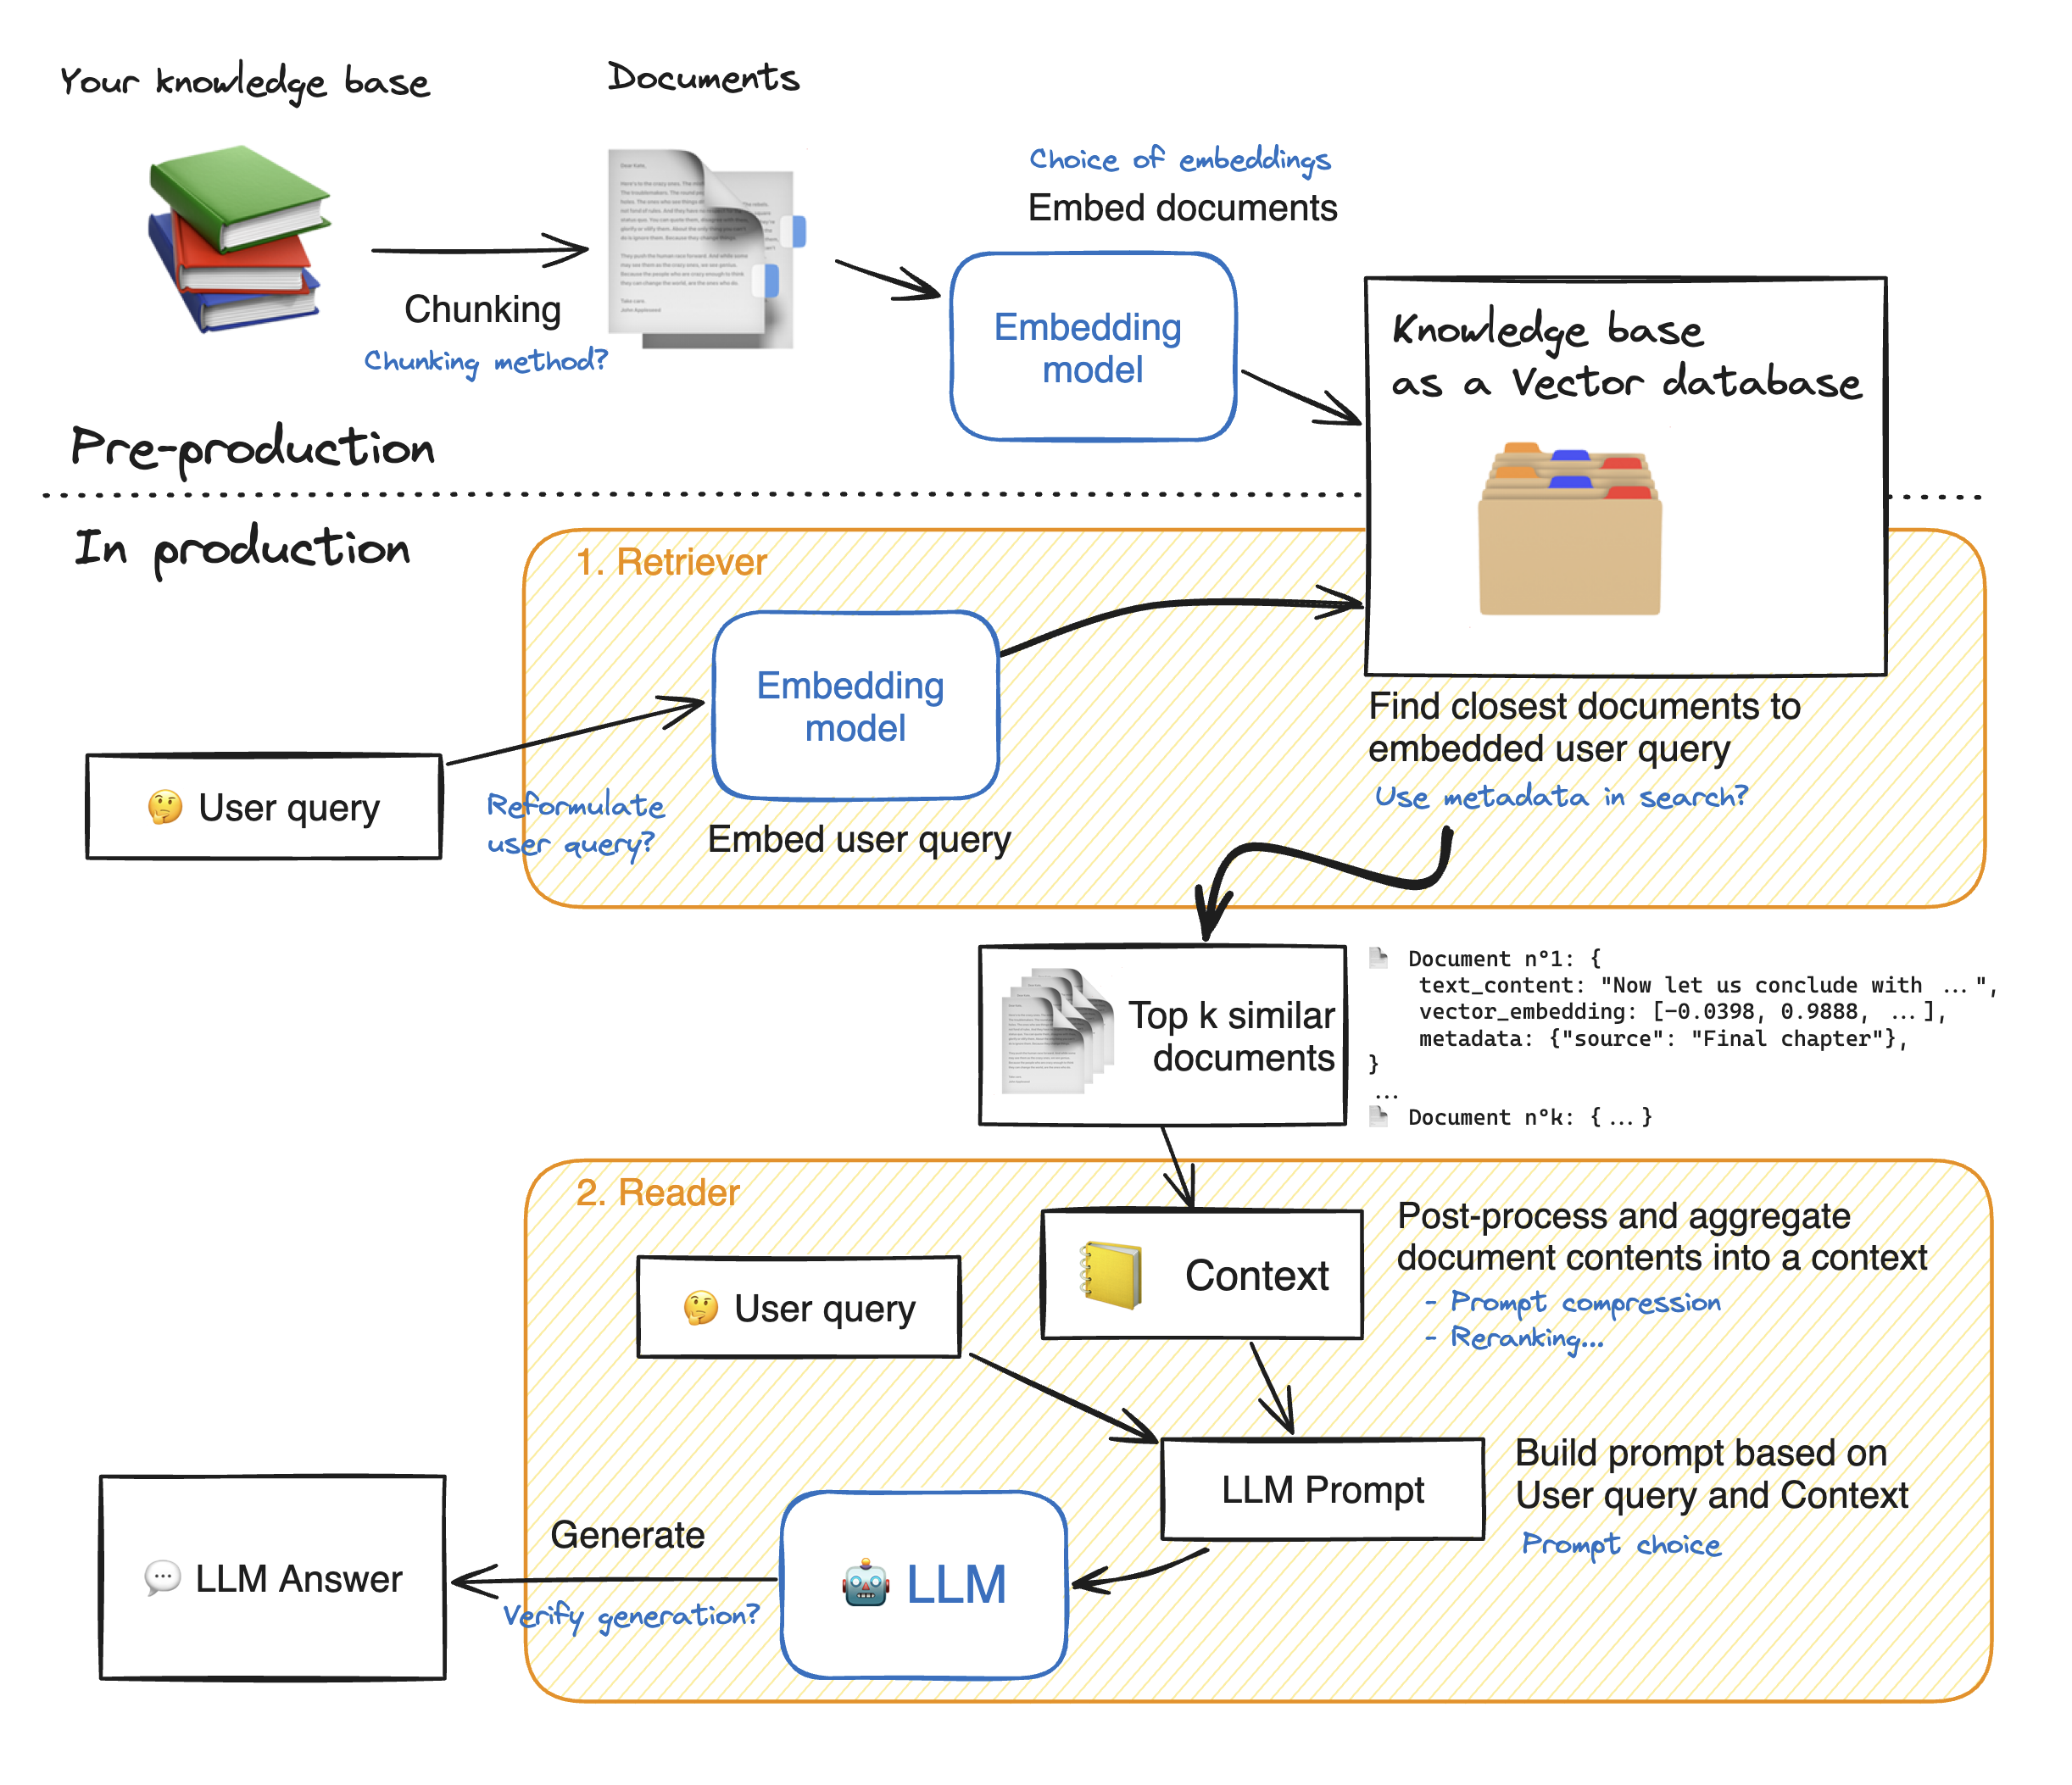
\includegraphics[width=\textwidth]{RAG_workflow.png}
\caption{Basic RAG pipeline~\cite{rag_pipeline_image}}
\end{figure}

The RAG pipeline explains how LLMs generate accurate answers using external
knowledge sources. The process begins with collecting documents from various
sources, forming a comprehensive knowledge base. Once gathered, the data is
divided into smaller segments called chunks, allowing efficient
processing and retrieval. Each chunk is then converted into a numerical
representation called an embedding, which transforms text into
vectors stored in a vector database.

When a user submits a query, the system converts it into a vector using the
same embedding process and retrieves the most relevant chunks. These chunks
are combined into a context passed alongside the user query to the LLM,
enabling it to produce responses that are more accurate, coherent, and less
prone to hallucinations.

%-------------------------------------------------------------
\subsubsection{a- RAG Use Cases}
%-------------------------------------------------------------

RAG techniques are versatile and have been applied across multiple real-world
domains. Their main advantages are the following:

\begin{itemize}
  \item \textbf{Dynamic and updated information:} RAG allows LLMs to deliver
        accurate and up-to-date responses by incorporating real-time external
        information that would otherwise fall outside their training knowledge.
  \item \textbf{Reduced errors:} By providing relevant context at inference
        time, RAG significantly reduces hallucinations and factual mistakes,
        leading to more trustworthy outputs.
  \item \textbf{Efficient and cost-effective:} RAG indexes data and stores
        it in a vector database, making correct information readily accessible
        without requiring costly model retraining.
  \item \textbf{Source attribution:} RAG can provide citations or references
        for the information it uses, increasing transparency and making
        responses more verifiable for end users.
  \item \textbf{Scalability:} RAG can handle large volumes of information
        and adapt to new domains by simply extending the knowledge base,
        without modifying the underlying model.
\end{itemize}

Building a RAG system requires choosing the right orchestration framework.
The following subsection compares the two main options considered for
Ask-Jade.

%-------------------------------------------------------------
\subsection{Different Technologies: LlamaIndex vs LangChain}
%-------------------------------------------------------------

LlamaIndex and LangChain are two popular frameworks used to build
applications based on Large Language Models, especially RAG systems.
LlamaIndex is mainly focused on document indexing and information retrieval,
making it well suited for search-oriented and knowledge-based systems.
In contrast, LangChain is more adapted to building complex pipelines,
agents, and conversational chatbots through its large ecosystem of tools
and integrations. An important advantage of LlamaIndex is its compatibility
with LangChain modules and document processing tools such as Docling,
allowing the development of efficient and scalable RAG applications.
Table \textbf{2.4} compares the main characteristics,
advantages, and limitations of both frameworks.

\begin{table}[H]
\centering
\caption{Feature Comparison: LlamaIndex vs.\ LangChain}
\label{tab:llama_langchain}
\renewcommand{\arraystretch}{1.5}
\begin{tabular}{|p{4cm}|p{5.5cm}|p{5.5cm}|}
\hline
\textbf{Feature / Aspect} & \textbf{LlamaIndex} & \textbf{LangChain} \\
\hline

Overview &
A platform for structured document indexing and semantic retrieval,
designed for precise information access. &
A versatile framework for constructing LLM-based pipelines and
connecting external data sources. \\
\hline

Advantages &
Fast indexing, handles large-scale datasets, native Docling integration,
and optimised for document workflows. &
Supports multi-step workflows, easy LangSmith integration,
and strong community support. \\
\hline

Limitations &
Mainly focused on retrieval; less suitable for complex multi-step
tool chaining. &
Steeper learning curve and heavier configuration for simple
document-centric tasks. \\
\hline

\end{tabular}
\end{table}

Beyond the orchestration framework, the quality of a RAG system depends
heavily on the embedding model used to represent documents and queries.
The following subsection presents the available options and justifies
the choice made for Ask-Jade.

%-------------------------------------------------------------
\subsection{Choice of Embedding Model}
%-------------------------------------------------------------

Embedding models play a critical role in RAG systems, as they directly influence the quality of semantic retrieval and the relevance of generated responses. This subsection presents the most commonly used embedding models and the criteria considered for selecting the most suitable one for the Ask-Jade system.

\subsubsection{a- Popular Embedding Models for RAG Systems}

Embedding models are essential components in RAG systems. Their role is to
transform documents and user queries into dense vector representations that
capture semantic meaning, enabling efficient similarity search and accurate
retrieval of relevant information from large document collections.
Table~\ref{tab:embedding_popular} summarises some of the most commonly used
embedding models for RAG systems.

\begin{table}[H]
\centering
\caption{Popular Embedding Models for RAG Systems}
\label{tab:embedding_popular}
\begin{tabular}{|p{4cm}|p{3cm}|p{3cm}|p{5cm}|}
\hline
\textbf{Embedding Model} & \textbf{Provider} & \textbf{Type}
& \textbf{Key Strengths} \\
\hline

text-embedding-3-large &
OpenAI &
Dense Embedding &
High retrieval accuracy, strong multilingual support,
optimised for semantic search \\
\hline

BGE-M3 &
BAAI &
Hybrid / Multilingual &
Supports dense, sparse, and multi-vector retrieval with excellent
multilingual performance \\
\hline

E5-large-v2 &
Microsoft &
Dense Embedding &
Strong semantic similarity and efficient retrieval for general-purpose
RAG systems \\
\hline

Instructor-XL &
HKUNLP &
Instruction-based &
Task-oriented embeddings with good performance on domain-specific
retrieval \\
\hline

\end{tabular}
\end{table}

%-------------------------------------------------------------

\subsubsection{b- Criteria for Choosing the Right Embedding Model}

Choosing the right embedding model means selecting the model that best
satisfies the semantic retrieval requirements, multilingual capabilities,
and scalability constraints of the system. Table \textbf{2.6}
presents the main criteria used in this comparative study.

\begin{table}[H]
\centering
\caption{Embedding Model Selection Criteria}
\label{tab:embedding_criteria}
\begin{tabular}{|p{5cm}|p{9cm}|}
\hline
\textbf{Criteria} & \textbf{Description} \\
\hline

Retrieval Accuracy &
Ability to capture semantic similarity and retrieve the most relevant
documents \\
\hline

Multilingual Capability &
Support for multiple languages such as English, French, and Arabic \\
\hline

Domain Adaptability &
Capability to represent technical, legal, financial, or domain-specific
terminology accurately \\
\hline

Scalability &
Efficiency when handling large document collections and high query volumes \\
\hline

Embedding Type &
Support for dense, sparse, or hybrid embeddings depending on retrieval
strategy \\
\hline

Performance \& Efficiency &
Computation speed, memory usage, and inference cost for real-time
applications \\
\hline

Integration Compatibility &
Ease of integration with vector databases, LlamaIndex, and RAG pipelines \\
\hline

\end{tabular}
\end{table}

%-------------------------------------------------------------

\subsubsection{c- Discussion}

Based on the comparative analysis, \textbf{BGE-M3}~\cite{bge_m3}, developed
by the Beijing Academy of Artificial Intelligence (BAAI), was selected as
the embedding model due to its strong multilingual support, hybrid retrieval
approach combining dense, sparse, and multi-vector representations, and
state-of-the-art performance on multilingual retrieval benchmarks.
Table \textbf{2.7} summarises its key technical specifications.

\begin{table}[H]
\centering
\caption{BGE-M3 Technical Specifications}
\label{tab:bge_m3_specs}
\renewcommand{\arraystretch}{1.4}
\begin{tabular}{|l|l|}
\hline
\textbf{Property} & \textbf{Value} \\
\hline
Base architecture    & XLM-RoBERTa \\
\hline
Languages supported  & 100+ (including French, English, Arabic) \\
\hline
Max input length     & 8{,}192 tokens \\
\hline
Embedding dimension  & 1{,}024 \\
\hline
Retrieval modes      & Dense, Sparse (lexical), Multi-vector (ColBERT) \\
\hline
Benchmarks           & MIRACL (18 languages), MKQA (25 languages), MLDR \\
\hline
\end{tabular}
\end{table}

Figure \textbf{2.3} compares BGE-M3 with other embedding
models on standard multilingual retrieval benchmarks, namely MIRACL
(nDCG 10) and MKQA (Recall 100), which evaluate ranking quality and
cross-lingual retrieval effectiveness respectively.

\begin{figure}[H]
\centering
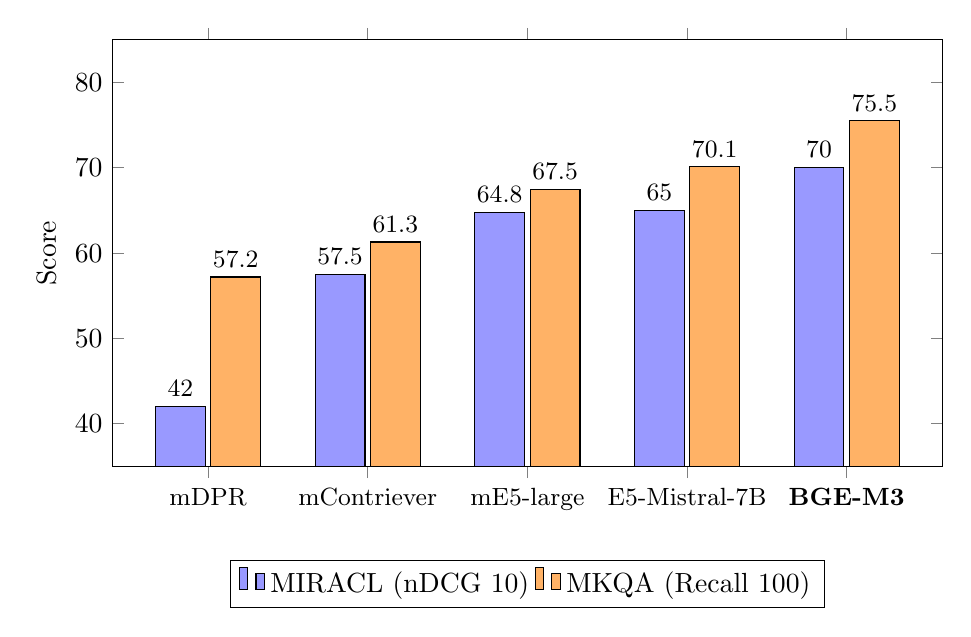
\begin{tikzpicture}
\begin{axis}[
    ybar,
    bar width=18pt,
    width=\textwidth,
    height=7cm,
    enlarge x limits=0.15,
    ylabel={Score},
    ymin=35, ymax=85,
    xtick=data,
    xticklabels={
        mDPR,
        mContriever,
        mE5-large,
        E5-Mistral-7B,
        \textbf{BGE-M3}
    },
    xticklabel style={font=\small},
    nodes near coords,
    nodes near coords align={above},
    every node near coord/.append style={font=\small},
    legend style={at={(0.5,-0.22)}, anchor=north, legend columns=2},
    legend cell align=left,
]
\addplot[fill=blue!40] coordinates {
    (1,42.0) (2,57.5) (3,64.8) (4,65.0) (5,70.0)
};
\addplot[fill=orange!60] coordinates {
    (1,57.2) (2,61.3) (3,67.5) (4,70.1) (5,75.5)
};
\legend{MIRACL (nDCG 10), MKQA (Recall 100)}
\end{axis}
\end{tikzpicture}
\caption{Comparison of embedding models on multilingual retrieval benchmarks.}
\label{fig:bge_m3_benchmark}
\end{figure}

The results confirm that BGE-M3 consistently outperforms competing models
on both benchmarks, demonstrating its effectiveness for multilingual and
cross-lingual retrieval tasks. Its scalability, efficient performance, and
native compatibility with LlamaIndex and vector databases make it well
suited for enterprise-level RAG applications.





%-------------------------------------------------------------
\section{Evaluation Framework}
\label{sec:eval_framework}
%-------------------------------------------------------------

Evaluating a RAG system requires dedicated metrics that measure both
retrieval and generation performance. In Ask-Jade, evaluation is performed
using the LLM-as-a-Judge paradigm, with all metrics tracked
through Langfuse~\cite{langfuse}.

%-------------------------------------------------------------
\subsection{LLM-as-a-Judge}
\label{sec:llm_as_judge}
%-------------------------------------------------------------
LLM-as-a-Judge offers several advantages and limitations that are important to consider when using it as an evaluation mechanism for RAG systems.

\subsubsection{a- Presentation}

LLM-as-a-Judge is an evaluation approach where a Large Language Model
acts as an automated evaluator for AI-generated responses. Instead of
relying on exact matching or token overlap, the judge LLM evaluates
responses using criteria such as relevance, coherence, faithfulness,
and factual accuracy.

This approach addresses the scalability limitations of human evaluation,
since manually annotating large numbers of query-answer pairs is costly
and time-consuming. A judge LLM can perform these evaluations
automatically at scale with strong correlation to human judgement~\cite{zheng2023judging}.

%-------------------------------------------------------------
\subsubsection{b- How It Works}

The judge LLM receives a structured prompt that includes:

\begin{enumerate}
  \item The \textbf{user query} the original question submitted
        by the user.
  \item The \textbf{retrieved context} the document chunks surfaced
        by the retrieval pipeline.
  \item The \textbf{generated answer} the response produced by the
        system under evaluation.
  \item An \textbf{evaluation rubric} explicit scoring criteria
        and instructions that define what constitutes a good or poor
        response.
\end{enumerate}

The judge then returns a score, a verdict (e.g.\ pass / fail), or a
detailed rationale explaining its assessment. Depending on the metric,
a reference answer may also be provided for comparison.


%-------------------------------------------------------------
\subsubsection{c- Advantages and Limitations}

LLM-as-a-Judge offers several advantages over traditional automated metrics. Table \textbf{2.8} presents a summary of its main advantages and limitations.

\begin{table}[H]
\centering
\caption{Advantages and Limitations of LLM-as-a-Judge}
\label{tab:llm_judge_adv_lim}
\renewcommand{\arraystretch}{1.3}
\begin{tabular}{|p{6cm}|p{6cm}|}
\hline
\textbf{Advantages} & \textbf{Limitations} \\
\hline

Semantic understanding: Evaluates meaning instead of surface form; robust to paraphrasing. 
&
Judge bias: May favour outputs similar to its own style. \\
\hline

Scalability: Automatically evaluates large datasets without human annotation. 
&
Positional bias: May prefer first or longer responses regardless of quality. \\
\hline

Alignment: Correlates well with human judgments in open-ended tasks. 
&
Cost: Requires API calls, increasing operational cost. \\
\hline

Flexibility: Adaptable evaluation rubrics for different domains. 
&
Non-determinism: Scores may vary across runs. \\
\hline

\end{tabular}
\end{table}

These limitations can be mitigated by using a judge model distinct from the generation model, fixing the evaluation temperature to zero to maximise reproducibility, and averaging scores over multiple runs when variance is a concern.




%-------------------------------------------------------------
\subsection{Retrieval Metrics}
%-------------------------------------------------------------
The following subsections introduce the metrics used to evaluate the quality of the retrieved context in terms of relevance, completeness, and factual correctness.
 
\subsubsection{a- Context Relevance}
 
Context Relevance measures whether the retrieved chunks are useful for
answering the user query. A high score indicates that the retrieved
context contains mostly relevant information, with little noise.
 
\begin{equation}
\text{Context Relevance} =
\frac{\text{Number of relevant retrieved sentences}}
     {\text{Total number of retrieved sentences}}
\label{eq:context_relevance}
\end{equation}
 
\textbf{Range:} $[0,\,1]$. A score close to 1 means the retriever
returns highly focused and pertinent content. A low score indicates
that the retrieved context contains too much irrelevant information.
 
%-------------------------------------------------------------
 
\subsubsection{b- Context Recall}
 
Context Recall measures the completeness of the retrieval: whether the
system successfully finds all the information needed to generate a
correct answer.
 
\begin{equation}
\text{Context Recall} =
\frac{\text{Relevant information successfully retrieved}}
     {\text{Total relevant information that should be retrieved}}
\label{eq:context_recall}
\end{equation}
 
\textbf{Range:} $[0,\,1]$. A low score indicates that important
information is missing from the retrieved context, which may lead to
incomplete or inaccurate answers.
 
%-------------------------------------------------------------
 
\subsubsection{c- Context Correctness}
 
Context Correctness evaluates whether the retrieved context is not only
complete but also factually accurate and correctly aligned with the
ground truth. Unlike Context Recall, which measures coverage, Context
Correctness penalises cases where retrieved chunks contain misleading
or incorrect information, even if they are topically relevant.
 
\begin{equation}
\text{Context Correctness} =
\frac{\text{Number of correctly retrieved and factually accurate chunks}}
     {\text{Total number of retrieved chunks}}
\label{eq:context_correctness}
\end{equation}
 
\textbf{Range:} $[0,\,1]$. A high score confirms that the retrieved
context is both relevant and factually reliable, providing a solid
foundation for accurate answer generation.
 
With retrieval quality defined, the following subsection introduces the
metrics used to evaluate the generation stage.
 
%-------------------------------------------------------------
\subsection{Generation Metrics}
%-------------------------------------------------------------

This subsection introduces the set of metrics used to assess the quality of the generated answers with respect to user intent, factual consistency, and response usefulness.
 
\subsubsection{a- Relevance}
 
Relevance measures the overall semantic alignment between the generated
answer and the user's query, independently of any reference answer.
It assesses whether the response directly and appropriately addresses
the intent behind the question.
 
\begin{equation}
\text{Relevance} =
\cos\!\left(\mathbf{q},\, \mathbf{a}\right)
\label{eq:relevance}
\end{equation}
 
where $\mathbf{q}$ is the embedding of the user query and $\mathbf{a}$
is the embedding of the generated answer.
 
\textbf{Range:} $[0,\,1]$. A high score indicates that the answer is
semantically close to the query and directly addresses the user's intent.
 
%-------------------------------------------------------------
 
\subsubsection{b- Answer Relevance}
 
Answer Relevance provides a more fine-grained measure of relevance by
generating $n$ candidate questions from the answer and measuring their
average cosine similarity to the original query embedding. This approach
penalises answers that are partially off-topic or introduce unnecessary
information.
 
\begin{equation}
\text{Answer Relevance} =
\frac{1}{n} \sum_{i=1}^{n}
\cos\!\left(\mathbf{q},\, \hat{\mathbf{q}}_i\right)
\label{eq:answer_relevance}
\end{equation}
 
where $\mathbf{q}$ is the embedding of the original question and
$\hat{\mathbf{q}}_i$ are the embeddings of the $n$ candidate questions
generated from the answer.
 
\textbf{Range:} $[0,\,1]$. A low score indicates that the answer
diverts from the user's intent or contains extraneous content.
 
%-------------------------------------------------------------
 
\subsubsection{c- Faithfulness}
 
Faithfulness checks whether every statement in the generated answer is
supported by the retrieved context. It measures the factual consistency
between the answer and its sources, independently of whether the
context itself is correct.
 
\begin{equation}
\text{Faithfulness} =
\frac{\text{Number of statements in the answer supported by the context}}
     {\text{Total number of statements in the generated answer}}
\label{eq:faithfulness}
\end{equation}
 
\textbf{Range:} $[0,\,1]$. A score of 1 means the answer is entirely
grounded in the retrieved documents with no unsupported claims.
A low score indicates that the model introduces information not present
in the context.
 
%-------------------------------------------------------------
 
\subsubsection{d- Hallucination}
 
Hallucination is defined as the complement of Faithfulness. It quantifies
the proportion of generated statements that cannot be verified in the
retrieved context, and therefore may represent fabricated or misleading
information.
 
\begin{equation}
\text{Hallucination} = 1 - \text{Faithfulness}
\label{eq:hallucination}
\end{equation}
 
\textbf{Range:} $[0,\,1]$. The objective is to minimise this score.
A high hallucination rate indicates that the model generates information
that is not grounded in the source documents, which undermines the
reliability of the system.
 
%-------------------------------------------------------------
 
\subsubsection{e- Answer Correctness}
 
Answer Correctness evaluates the overall quality of the generated answer
by comparing it to a reference answer. It combines two complementary
measures: factual overlap, computed using the F1 score at the token level,
and semantic similarity, computed using the cosine similarity of the
answer embeddings.
 
\begin{equation}
\text{Answer Correctness} =
w_1 \cdot F_1\!\left(a,\, a^{*}\right) +
w_2 \cdot \cos\!\left(\mathbf{a},\, \mathbf{a}^{*}\right)
\label{eq:answer_correctness}
\end{equation}
 
where:
\begin{itemize}
  \item $a$ is the generated answer and $a^{*}$ is the reference answer,
  \item $w_1$ and $w_2$ are weighting coefficients
        (typically $w_1 = w_2 = 0.5$),
  \item $F_1(a, a^{*})$ measures token-level factual overlap between
        the generated and reference answers,
  \item $\cos(\mathbf{a}, \mathbf{a}^{*})$ measures the semantic
        similarity between the embeddings of the two answers.
\end{itemize}
 
\textbf{Range:} $[0,\,1]$. A high score means the generated answer
is both factually and semantically close to the expected answer.
A low score may indicate missing facts, incorrect statements,
or a semantically divergent response.
 
%-------------------------------------------------------------
 
\subsubsection{f- Helpfulness and Conciseness}
 
Beyond factual accuracy, additional metrics evaluate the practical
quality of the generated answer.
 
Helpfulness measures whether the answer is useful and complete
for the user's needs, while Conciseness evaluates whether the
response is brief and focused without unnecessary information.
Both metrics are scored in $[0,\,1]$ by the judge LLM.





%-------------------------------------------------------------
\subsection{Summary of Evaluation Metrics}
%-------------------------------------------------------------
 
Table \textbf{2.9} summarises all evaluation metrics, their categories, and their target thresholds, which define the minimum acceptable performance levels for each metric.
 
\begin{table}[H]
\centering
\caption{Summary of evaluation metrics}
\label{tab:eval_summary}
\renewcommand{\arraystretch}{1.4}
\begin{tabular}{|p{3.5cm}|p{2.5cm}|p{6cm}|p{2cm}|}
\hline
\textbf{Metric} & \textbf{Category} & \textbf{What it measures} & \textbf{Target} \\
\hline
Context Relevance &
Retrieval &
Proportion of relevant sentences among all retrieved sentences &
$\geq 0.80$ \\
\hline
Context Recall &
Retrieval &
Completeness of the retrieved information relative to what is needed &
$\geq 0.80$ \\
\hline
Context Correctness &
Retrieval &
Factual accuracy and alignment of retrieved chunks with the ground truth &
$\geq 0.75$ \\
\hline
Relevance &
Generation &
Overall semantic alignment of the generated answer with the user's query &
$\geq 0.85$ \\
\hline
Answer Relevance &
Generation &
Fine-grained alignment of the answer with the query via candidate question generation &
$\geq 0.80$ \\
\hline
Faithfulness &
Generation &
Proportion of answer statements supported by the retrieved context &
$\geq 0.80$ \\
\hline
Hallucination &
Generation &
Proportion of answer statements not supported by the context &
$\leq 0.15$ \\
\hline
Answer Correctness &
Generation &
Factual and semantic match between the generated and reference answers &
$\geq 0.75$ \\
\hline
Helpfulness &
Generation &
Overall usefulness of the answer for the user's needs &
$\geq 0.75$ \\
\hline
Conciseness &
Generation &
Appropriateness of answer length and focus without unnecessary verbosity &
$\geq 0.75$ \\
\hline
\end{tabular}
\end{table}







\section{Conclusion}
In this chapter we have provided an overview of the core technologies that are used in modern retrieval-based question answering applications. Large Language Models provide powerful language understanding but are still constrained by hallucinations and

ancient wisdom. Retrieval-Augmented Generation (RAG) solves these problems by providing answers based on external documents. Using BGE-M3 for embedding and LLM-as-a-Judge for evaluation gives us a good basis to create reliable and accurate AI-driven solutions.